\documentclass[aspectratio=169,11pt]{beamer}
\usepackage[T1]{fontenc}
\usepackage[utf8]{inputenc}
\usepackage{lmodern}
\usepackage{array,booktabs}
\usepackage{listings}
\usepackage{tikz}
\usetikzlibrary{positioning,arrows.meta,fit,backgrounds,decorations.pathreplacing}

% Same TikZ styles as slides.tex, so the report's diagrams render unchanged.
\tikzset{box/.style={draw=black!65,rounded corners=3pt,minimum height=9mm,
 align=center,font=\small,inner sep=5pt},
 inputbox/.style={box,fill=blue!10},processbox/.style={box,fill=green!12},
 outputbox/.style={box,fill=orange!20},arrow/.style={-{Stealth[length=2mm]},thick},
 message/.style={arrow,dashed,draw=orange!85!black}}
\tikzset{card/.style={draw=black!25,fill=#1,rounded corners=4pt,minimum width=44mm,minimum height=30mm,align=center,inner sep=5pt}}
\newcommand{\secnum}[1]{}
\newcommand{\diagram}[1]{\resizebox{\linewidth}{!}{\input{diagrams/#1.tex}}}
% Shared encoding figure (diagrams/offset-encoding.tex).
\newcommand{\encodingfig}[1]{\begingroup\def\encodingextra{#1}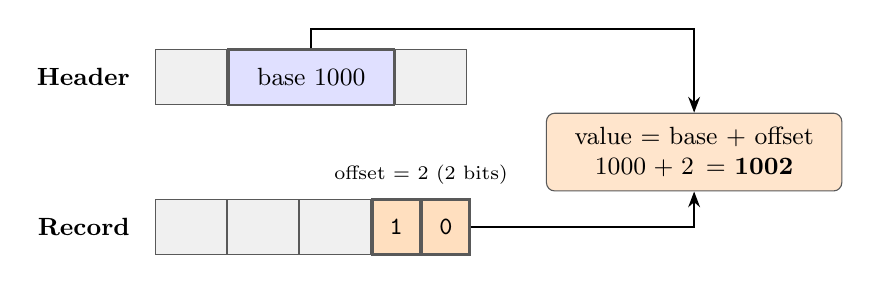
\begin{tikzpicture}[
  cell/.style={draw=black!65,minimum height=7mm,font=\small,inner sep=2pt},
  other/.style={cell,minimum width=9mm,fill=black!6},
  bit/.style={cell,minimum width=6mm,fill=orange!25,line width=0.9pt,font=\small\ttfamily}]
\node[font=\small\bfseries,anchor=east] at (-0.2,0) {Header};
\node[other,anchor=west] (h1) at (0,0) {};
\node[cell,fill=blue!12,line width=0.9pt,minimum width=21mm,right=0mm of h1] (base) {base 1000};
\node[other,right=0mm of base] (h2) {};
\node[font=\small\bfseries,anchor=east] at (-0.2,-1.9) {Record};
\node[other,anchor=west] (r1) at (0,-1.9) {};
\node[other,right=0mm of r1] (r2) {};
\node[other,right=0mm of r2] (r3) {};
\node[bit,right=0mm of r3] (f1) {1};
\node[bit,right=0mm of f1] (f2) {0};
\node[font=\scriptsize,above=0.5mm of f1.north east] {offset = 2 (2 bits)};
\node[outputbox,text width=34mm,right=10mm of h2.east,yshift=-9.5mm] (value) {value = base + offset\\$1000 + 2 =$ \textbf{1002}};
\draw[arrow] (base.north) -- ++(0,2.5mm) -| (value.north);
\draw[arrow] (f2.east) -| (value.south);
% Optional annotation used by the validation slide.
\ifdefined\encodingextra\encodingextra\fi
\end{tikzpicture}
\endgroup}

\definecolor{navy}{HTML}{1B2340}
\definecolor{gold}{HTML}{D4A537}
\definecolor{cream}{HTML}{F6EDCF}
\setbeamercolor{frametitle}{fg=navy}
\setbeamercolor{title}{fg=navy}
\setbeamercolor{structure}{fg=navy}
\setbeamercolor{item}{fg=gold!85!black}
\setbeamerfont{frametitle}{series=\bfseries,size=\Large}
\setbeamertemplate{navigation symbols}{}
\setbeamertemplate{footline}{\hfill\scriptsize\color{black!50}
 DPHPC 2026 · Self-describing GOAL traces\quad\insertframenumber\hspace*{4mm}\vspace*{2mm}}
\setbeamertemplate{itemize items}[circle]

\lstset{basicstyle=\ttfamily\scriptsize,columns=fullflexible,keepspaces=true,
 breaklines=true,showstringspaces=false,frame=single,rulecolor=\color{black!18},
 backgroundcolor=\color{black!3},xleftmargin=3pt,xrightmargin=3pt}

\newcolumntype{L}[1]{>{\raggedright\arraybackslash}p{#1}}
\newcommand{\highlight}[1]{\colorbox{cream}{\parbox{\dimexpr\linewidth-2\fboxsep}{\small #1}}}
\newcommand{\source}[1]{{\scriptsize\color{black!55}\par\vspace{2mm}#1\par}}
% Step title slide: the four-step pipeline with this step highlighted, and the question it answers.
\newcommand{\stepframe}[3]{%
\begin{frame}
\vfill
{\centering
{\usebeamercolor[fg]{title}\large\bfseries Step #1\par}
\vspace{1mm}
{\usebeamercolor[fg]{title}\huge\bfseries #2\par}
\vspace{3mm}
{\color{black!60}#3\par}
\vspace{9mm}
\def\activestep{#1}%
\resizebox{0.85\linewidth}{!}{% The pipeline with the four design steps, numbered in presentation order.
% \activestep (0 = none) highlights one step and fades the rest.
\providecommand{\activestep}{0}
\begin{tikzpicture}[
  stepstate/.code={\ifnum\activestep=0\relax\else
    \ifnum#1=\activestep\relax\tikzset{draw=gold!85!black,line width=1.6pt}\else\tikzset{opacity=0.3}\fi\fi},
  stepbadge/.style={circle,fill=gold,text=white,font=\small\bfseries,inner sep=0pt,minimum size=6mm},
  steplabel/.style={font=\small,align=center,text width=30mm}]
\node[inputbox,text width=22mm,stepstate=0] (t) at (0,0) {GOAL text};
\node[processbox,text width=22mm,stepstate=3] (c) at (3.9,0) {Converter\\\footnotesize\texttt{txt2bin}};
\node[outputbox,text width=22mm,stepstate=1] (f) at (7.8,0) {Binary file};
\node[processbox,text width=22mm,stepstate=2] (r) at (11.7,0) {Reader};
\node[outputbox,text width=22mm,stepstate=4] (s) at (15.6,0) {Simulator\\\footnotesize LogGOPSim};
\foreach \a/\b in {t/c,c/f,f/r,r/s} \draw[arrow,stepstate=-1] (\a)--(\b);
\foreach \target/\n/\label in {
    f/1/{Self-describing\\format\\[1mm]{\scriptsize\color{black!60}the header describes\\every field}},
    r/2/{JIT\\decoding\\[1mm]{\scriptsize\color{black!60}a decoder compiled\\for each file}},
    c/3/{Parallel\\conversion\\[1mm]{\scriptsize\color{black!60}ranks parsed\\on all cores}},
    s/4/{Lazy\\decoding\\[1mm]{\scriptsize\color{black!60}decode a node\\when it runs}}} {
  \node[stepbadge,below=5mm of \target,stepstate=\n] (n\n) {\n};
  \node[steplabel,below=1mm of n\n,stepstate=\n,draw=none] {\label};
}
\end{tikzpicture}
}\par}
\vfill
\end{frame}}

\title{Self-describing GOAL traces for LogGOPSim}
\subtitle{DPHPC 2026 progress presentation}
\author{Joshua Durrant, Alexander Falter, Samuel Garcin, Mykhaylo Gershman}
\date{Supervised by Timo Schneider \\ 17.11.26}

\begin{document}

\begin{frame}
\titlepage
\end{frame}

% ================================================================ old design

\begin{frame}{LogGOPSim today}
\small
LogGOPSim predicts how long an MPI program runs. Input: per rank, a graph of sends, receives and computations. Output: the predicted runtime.
\vspace{5mm}

{\centering\diagram{original-overview}\par}
\vspace{5mm}
\begin{itemize}
\item \texttt{txt2bin} converts the text schedule once; each simulation then reads the binary file.
\item The reader is built into LogGOPSim and knows the record layout by heart.
\end{itemize}
\end{frame}

\begin{frame}{A schedule is a dependency graph}
\begin{columns}[c]
\begin{column}{0.45\textwidth}
\centering\resizebox{\linewidth}{!}{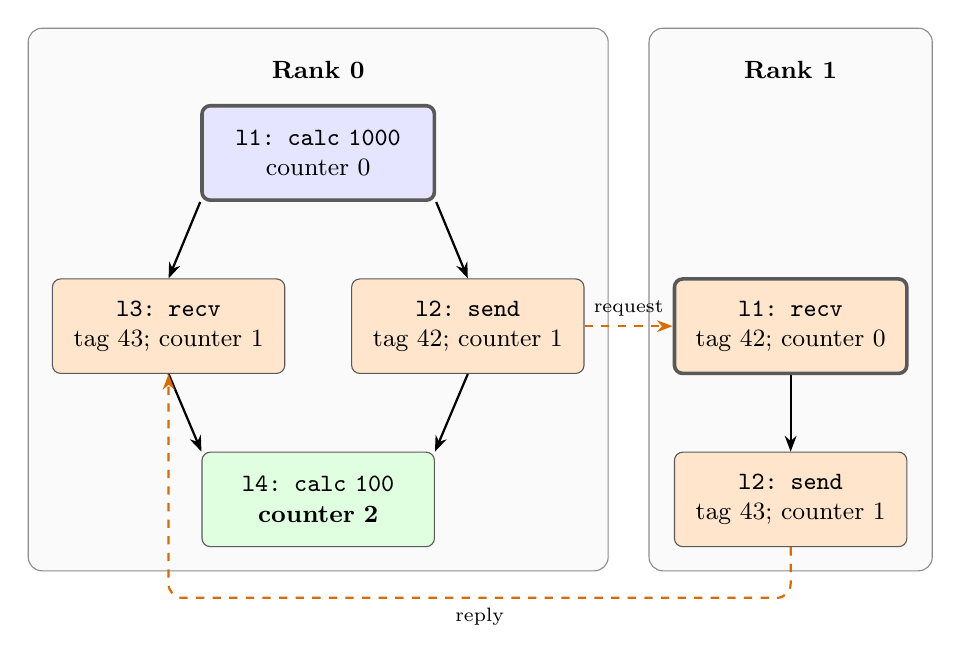
\begin{tikzpicture}[
  op/.style={inputbox,text width=26mm,minimum height=12mm,inner sep=5pt,font=\small},
  root/.style={line width=1.3pt}]
\node[font=\small\bfseries] (rank0title) at (0,1.05) {Rank 0};
\node[font=\small\bfseries] (rank1title) at (6,1.05) {Rank 1};
\node[op,root] (a) at (0,0) {\texttt{l1: calc 1000}\\counter 0};
\node[op,fill=orange!20] (b) at (1.9,-2.2) {\texttt{l2: send}\\tag 42; counter 1};
\node[op,fill=orange!20] (c) at (-1.9,-2.2) {\texttt{l3: recv}\\tag 43; counter 1};
\node[op,fill=green!12] (d) at (0,-4.4) {\texttt{l4: calc 100}\\\textbf{counter 2}};
\node[op,root,fill=orange!20] (e) at (6,-2.2) {\texttt{l1: recv}\\tag 42; counter 0};
\node[op,fill=orange!20] (f) at (6,-4.4) {\texttt{l2: send}\\tag 43; counter 1};
\begin{scope}[on background layer]
\node[draw=black!45,fill=black!2,rounded corners=5pt,inner sep=3mm,
  fit=(rank0title)(a)(b)(c)(d)] {};
\node[draw=black!45,fill=black!2,rounded corners=5pt,inner sep=3mm,
  fit=(rank1title)(e)(f)] {};
\end{scope}
\draw[arrow] (a.south west) -- (c.north);
\draw[arrow] (a.south east) -- (b.north);
\draw[arrow] (c.south) -- (d.north west);
\draw[arrow] (b.south) -- (d.north east);
\draw[arrow] (e.south) -- (f.north);
\draw[message] (b.east) -- node[above,font=\scriptsize] {request} (e.west);
\draw[message,rounded corners=5pt] (f.south) -- (6,-5.65)
  -- node[below,font=\scriptsize] {reply} (-1.9,-5.65) -- (c.south);
\end{tikzpicture}
}
\end{column}
\begin{column}{0.52\textwidth}
\small
\begin{itemize}
\item Each rank is a graph of \texttt{calc}, \texttt{send} and \texttt{recv} nodes.
\item A node's \textbf{counter} says how many nodes it still waits for. Roots start at 0.
\item The simulator runs ready nodes with LogGOPS costs ($L$, $o$, $g$, $G$), then decrements the counters of their dependents.
\item A dependent whose counter reaches 0 becomes ready.
\item Output: the time at which each rank finishes.
\end{itemize}
\end{column}
\end{columns}
\end{frame}

\begin{frame}{The problem: a fixed 39-byte record}
\diagram{legacy-record}
\vspace{4mm}
\begin{itemize}
\item \textbf{Wasteful:} every field at full width, whatever values occur. Most traces need 2--4 bytes per node.
\item \textbf{Closed:} no room for extra information. ATLAHS hides the GPU in \texttt{nic} and packs five numbers into the tag; a wrong guess gives wrong results silently.
\item \textbf{Hard-wired:} each simulator needs its own copy of the byte offsets.
\end{itemize}
\end{frame}

\begin{frame}{Our design in four steps}
\centering\vfill
\diagram{design-steps}
\vfill
\par\raggedright
\highlight{Step 1 solves the problem. Steps 2--4 make sure the new format costs nothing: reading, converting and simulating get faster, not slower.}
\end{frame}

% ================================================================ step 1

\stepframe{1}{Self-describing format}{The file says what is in it}

\begin{frame}{The file describes itself}
\diagram{file-sections}
\vspace{4mm}
\begin{itemize}
\item The \textbf{schema header} lists every field: name, type, bit position, width, base. A reader needs no built-in knowledge of the layout.
\item All records of a file share one layout, so node $i$ of a rank is at \mbox{\texttt{rank\_start + i $\times$ record\_size}}, without scanning.
\item A new magic number tells the formats apart: legacy files stay readable through the same reader.
\end{itemize}
\end{frame}

\begin{frame}{Each field gets only the bits it needs}
\begin{columns}[c]
\begin{column}{0.5\textwidth}
\centering\resizebox{\linewidth}{!}{\encodingfig{}}
\end{column}
\begin{column}{0.47\textwidth}
\small
\begin{itemize}
\item Width from the field's largest value.
\item \textbf{Offset encoding:} the header stores the smallest value (the base), records store the offset.
\item A constant field takes \textbf{0 bits}: its value lives only in the header.
\item bcast\_64k: 39 $\to$ 4 bytes per node.
\end{itemize}
\end{column}
\end{columns}
\vspace{6mm}
\highlight{\textbf{In the grand picture:} the layout depends on every value in the trace. The converter must see all values before writing (Step 3), and the reader must interpret the layout (Step 2).}
\end{frame}

\begin{frame}[fragile]{Custom fields: the ATLAHS case}
\begin{lstlisting}
before: l2: send 1024b to 1 tag 3050012001 cpu 0 nic 2
after:  l2: send 1024b to 1 tag 0 cpu 0 nic 0 stream_id 0 gpu_id 2 peer_gpu_id 2
            chunk_id 3 channel_id 5 sequence_id 12 message_kind 0 communicator_id 1
\end{lstlisting}
\vspace{3mm}
\begin{columns}[T]
\begin{column}{0.56\textwidth}
\small
\begin{itemize}
\item Custom fields are declared in TOML and treated like standard ones.
\item Each simulator binds only the fields it needs; a missing field or a value too large for its member fails at load time.
\item Explicit fields exposed and fixed two htsim bugs: messages sent to the wrong GPU, and different messages sharing a tag.
\end{itemize}
\end{column}
\begin{column}{0.4\textwidth}
\highlight{\centering Recorded Llama run, 5.7M operations:\\[1mm]{\Large\bfseries 54\% smaller}\\ with all eight extra fields}
\end{column}
\end{columns}
\end{frame}

% ================================================================ step 2

\stepframe{2}{JIT decoding}{A flexible format must not be slower to read}

\begin{frame}{Flexibility has a cost at read time}
\centering\vfill
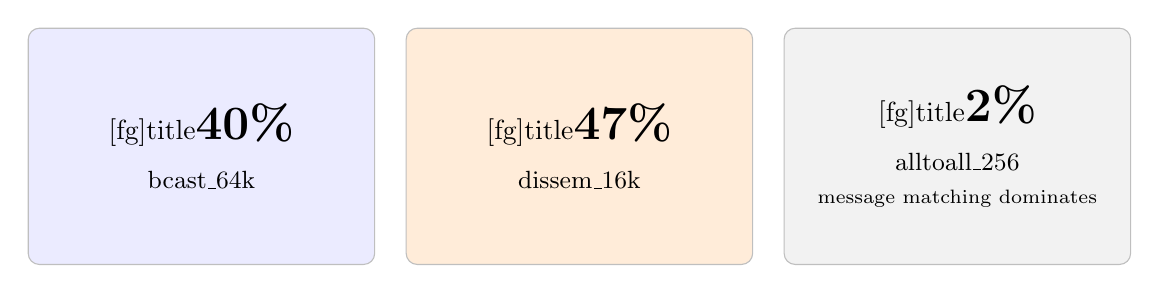
\begin{tikzpicture}
\node[card=blue!8] at (0,0) {{\usebeamercolor[fg]{title}\LARGE\bfseries 40\%}\\[2mm]\small bcast\_64k};
\node[card=orange!15] at (48mm,0) {{\usebeamercolor[fg]{title}\LARGE\bfseries 47\%}\\[2mm]\small dissem\_16k};
\node[card=black!5] at (96mm,0) {{\usebeamercolor[fg]{title}\LARGE\bfseries 2\%}\\[2mm]\small alltoall\_256\\\scriptsize message matching dominates};
\end{tikzpicture}
\vfill
\par\raggedright
\begin{itemize}
\item Share of the simulation time spent decoding, with the first, generic decoder.
\item Bit positions are known only when the file is opened, so it interpreted the header for every field of every node: look up position, shift, mask, add base, check range.
\end{itemize}
\end{frame}

\begin{frame}{Build the decoder once, run it for every node}
\centering\resizebox{!}{0.5\textheight}{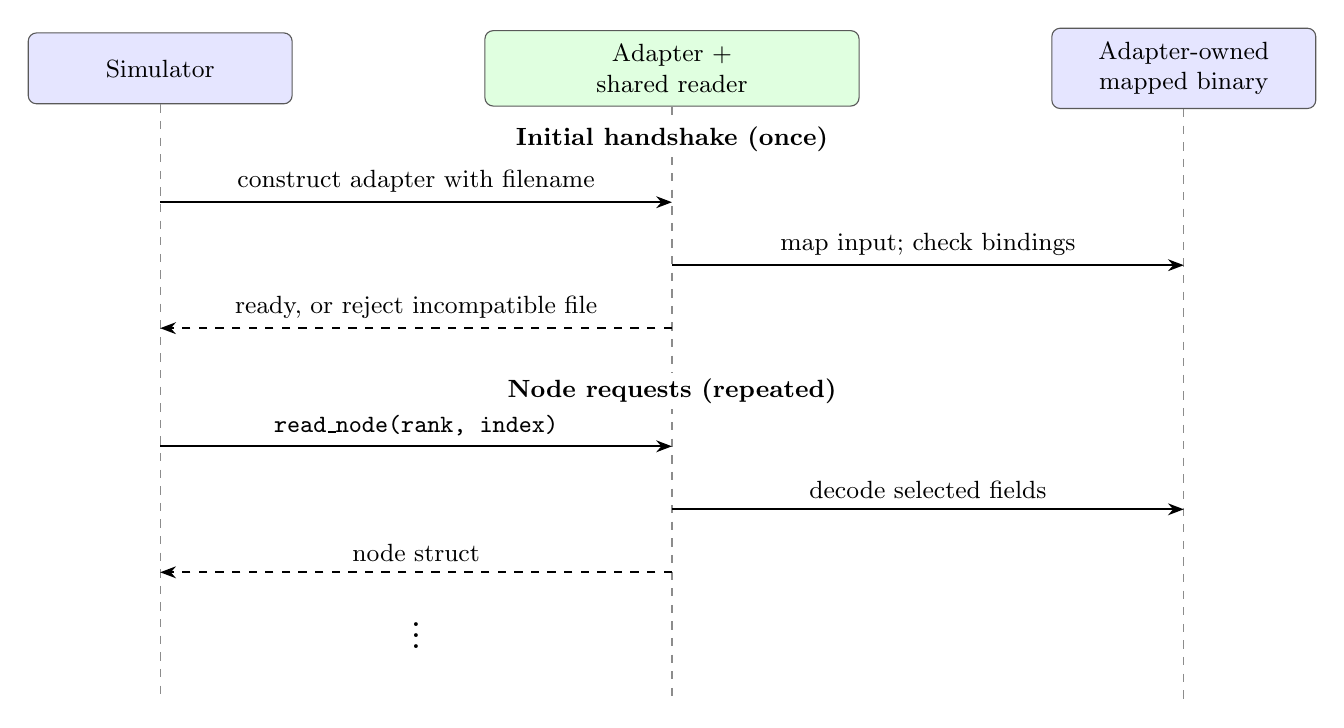
\begin{tikzpicture}
\node[inputbox,text width=30mm] (s) at (0,0) {Simulator};
\node[processbox,text width=44mm] (r) at (6.5,0) {Adapter +\\shared reader};
\node[inputbox,text width=30mm] (f) at (13,0) {Adapter-owned\\mapped binary};
\foreach \p in {s,r,f} \draw[dashed,black!45] (\p.south)--++(0,-7.5);
\node[font=\small\bfseries,fill=white,inner sep=2pt] at (6.5,-0.9) {Initial handshake (once)};
\draw[arrow] (0,-1.7)--node[above,font=\small]{construct adapter with filename}(6.5,-1.7);
\draw[arrow] (6.5,-2.5)--node[above,font=\small]{map input; check bindings}(13,-2.5);
\draw[arrow,dashed] (6.5,-3.3)--node[above,font=\small]{ready, or reject incompatible file}(0,-3.3);
\node[font=\small\bfseries,fill=white,inner sep=2pt] at (6.5,-4.1) {Node requests (repeated)};
\draw[arrow] (0,-4.8)--node[above,font=\small]{\texttt{read\_node(rank, index)}}(6.5,-4.8);
\draw[arrow] (6.5,-5.6)--node[above,font=\small]{decode selected fields}(13,-5.6);
\draw[arrow,dashed] (6.5,-6.4)--node[above,font=\small]{node struct}(0,-6.4);
\node[font=\Large,fill=white] at (3.25,-7.1) {$\vdots$};
\end{tikzpicture}
}
\par\raggedright\vspace{3mm}
\small
\begin{itemize}
\item \textbf{Once, when the file is opened:} take the fields the simulator binds, build a \textbf{decode plan} (one step per field: offset, shift, mask, base, destination), pick a runner.
\item \textbf{For every node:} the runner turns the record's bits into the simulator's node struct.
\end{itemize}
\end{frame}

\begin{frame}[fragile]{Compiled runners hard-code the layout}
\begin{columns}[T]
\begin{column}{0.46\textwidth}
\begin{lstlisting}
int decode(const u8* r, u8* const* t) {
  u64 w, c;
  // peer: 16 bits at bit 3
  memcpy(&w, r + 0x0, 8);
  c = (w >> 0x3) & 0xffff;
  store32(t[0] + 0x3c, c);
  // size: 0 bits, constant 1024
  store64(t[0] + 0x40, 0x400);
  // ... further fields
  return 1;
}
\end{lstlisting}
{\scriptsize\color{black!55}Generated C for bcast\_64k, abridged.\par}
\end{column}
\begin{column}{0.5\textwidth}
\small
\begin{itemize}
\item Every position and mask is a constant: no loop, no lookup.
\item \texttt{jit}: compiled with \texttt{cc}, cached on disk (about 340\,ms the first time).
\item \texttt{orc}: the same function in memory with LLVM (about 2.5\,ms).
\item \texttt{plan}: interpreter, the default and fallback.
\item Only numbers from the header go into the code, so a trace can't inject code.
\end{itemize}
\vspace{2mm}
\highlight{\texttt{jit}: 12--17\,ns per node, 2$\times$ the interpreter, within 6\% of code compiled ahead of time.}
\end{column}
\end{columns}
\end{frame}

% ================================================================ step 3

\stepframe{3}{Parallel conversion}{Converting is now two passes; make them use all cores}

\begin{frame}{Why conversion reads the input twice}
\diagram{conversion-overview}
\vspace{4mm}
\begin{itemize}
\item The layout must be fixed before the first record is written: if tags 0--7 fit in 3 bits but a later rank uses tag 1000, earlier records can't be widened.
\item \textbf{Pass 1} only collects statistics: each field's minimum and maximum, wildcards, counts.
\item \textbf{Pass 2} parses again and packs each rank with the final layout.
\item One rank's graph in memory at a time, so memory stays bounded.
\end{itemize}
\vspace{2mm}
\highlight{Pass 1 was one sequential scan through a \texttt{FILE*}: 22--38\,s on our largest traces.}
\end{frame}

\begin{frame}{Pass 1 in parallel: one rank per task}
\vspace{2mm}
{\centering\resizebox{0.8\linewidth}{!}{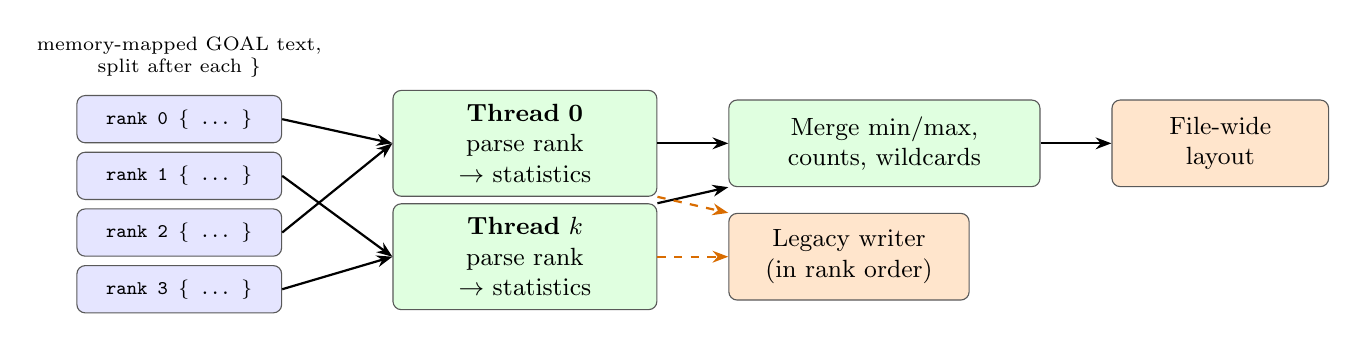
\begin{tikzpicture}[node distance=6mm and 9mm]
% The memory-mapped GOAL text, split after each rank block's closing brace.
\foreach \r/\y in {0/0,1/-1,2/-2,3/-3} {
  \node[inputbox,minimum width=26mm,minimum height=6mm,font=\scriptsize\ttfamily] (r\r) at (0,\y*0.72)
    {rank \r\ \{ \dots\ \}};
}
\node[font=\scriptsize,above=1mm of r0,align=center] {memory-mapped GOAL text,\\split after each \texttt{\}}};
% Threads parse whole ranks with the sequential scanner and keep their own statistics.
\node[processbox,text width=30mm,minimum height=11mm,right=14mm of r0.south east,anchor=west] (t0)
  {\textbf{Thread 0}\\parse rank $\to$ statistics};
\node[processbox,text width=30mm,minimum height=11mm,right=14mm of r2.south east,anchor=west] (t1)
  {\textbf{Thread $k$}\\parse rank $\to$ statistics};
\foreach \r/\t in {r0/t0,r1/t1,r2/t0,r3/t1} \draw[arrow] (\r.east)--(\t.west);
% Partial statistics are merged; legacy ranks are written in rank order.
\node[processbox,text width=36mm,minimum height=11mm,right=of t0] (m)
  {Merge min/max,\\counts, wildcards};
\node[outputbox,text width=24mm,minimum height=11mm,right=of m] (l) {File-wide\\layout};
\node[outputbox,text width=27mm,minimum height=11mm,right=of t1] (w)
  {Legacy writer\\(in rank order)};
\draw[arrow] (t0)--(m); \draw[arrow] (t1.north east)--(m.south west); \draw[arrow] (m)--(l);
\draw[message] (t0.south east)--(w.north west); \draw[message] (t1)--(w);
\end{tikzpicture}
}\par}
\vspace{5mm}
\begin{itemize}
\item In GOAL, ranks are independent blocks. The memory-mapped text is cut after each rank's closing brace (skipping comments).
\item OpenMP threads parse whole ranks with the unchanged scanner and keep their own statistics.
\item Minimum, maximum and counts merge in any order, so the result doesn't depend on the thread count. \texttt{txt2bin -{}-threads N}.
\end{itemize}
\end{frame}

\begin{frame}{Same result as before, and what it took}
\begin{columns}[T]
\begin{column}{0.48\textwidth}
\textbf{Identical to the sequential pass}
\small
\begin{itemize}
\item Same output bytes in both formats.
\item Same errors: the lowest invalid rank is reported, with its line number in the whole file.
\item 9 differential tests at 1, 2, 3 and 8 threads.
\item Pipes can't be mapped: they use the sequential reader.
\end{itemize}
\end{column}
\begin{column}{0.48\textwidth}
\textbf{Two bottlenecks found on the way}
\small
\begin{itemize}
\item The legacy writer remapped the whole output file for every rank. With threads, each unmap got expensive: 45\,s instead of 4\,s. Now each rank is appended with \texttt{pwrite}.
\item Threads waiting in \texttt{omp ordered} spin and starved the writer: 15\,s instead of under 1\,s. Now they sleep on a condition variable.
\end{itemize}
\end{column}
\end{columns}
\end{frame}

% ================================================================ step 4

\stepframe{4}{Lazy decoding}{Decode a node only when the simulator runs it}

\begin{frame}{Where the simulator spends memory}
\centering\diagram{lazy-flow}
\par\raggedright\vspace{5mm}
\small
\begin{itemize}
\item \textbf{Before:} counters are decremented in the memory-mapped file. The mapping is private, so the file stays reusable, but every page written is copied: a long run copies most of the file.
\item \textbf{Lazy:} counters move to a small array, ready nodes are indices, and each node is decoded once, when it runs.
\end{itemize}
\end{frame}

\begin{frame}[fragile]{Implementation}
\begin{columns}[T]
\begin{column}{0.6\textwidth}
\begin{lstlisting}[language=C++]
// A node finished: release its dependents.
for (auto i : dependents) {
  auto& c = counters_[i];  // remaining + 1
  if (c == 0)              // first use
    c = reader.read_dependency_count(rank, i) + 1;
  if (--c == 1)            // none left
    ready_.push_back(i);   // 4-byte index
}

// The simulator takes the ready nodes: decode now.
for (auto i : ready_)
  out.push_back(reader.read_node(rank, i));
\end{lstlisting}
{\scriptsize\color{black!55}From \texttt{SimulationSchedule.hpp}, simplified.\par}
\end{column}
\begin{column}{0.37\textwidth}
\small
\begin{itemize}
\item Counters are read from the file only on their first decrement: no extra pass over the file at startup.
\item 0 means ``not read yet'', so the stored value is the remaining count plus one.
\item Works for both formats and every decoder, through the same reader.
\item Opt-in flag \texttt{-{}-lazy-decoding}; the default is unchanged.
\end{itemize}
\end{column}
\end{columns}
\end{frame}

\begin{frame}{Same simulation, fewer copies}
\begin{columns}[T]
\begin{column}{0.48\textwidth}
\textbf{Correctness}
\small
\begin{itemize}
\item The full \texttt{-v} event log is identical in both modes: every operation at the same simulated time.
\item Checked on dissemination, ResNet and ring traces (14.7M--72.8M log lines), both formats.
\item The trace file is never written, so it can be shared by concurrent runs.
\end{itemize}
\end{column}
\begin{column}{0.48\textwidth}
\textbf{Trade-offs}
\small
\begin{itemize}
\item The counter array is 4\,B per node, allocated at startup: 1 billion nodes need 4\,GB, still far less than the page copies it replaces.
\item Not combinable with \texttt{-{}-save-mem}, which exists only to write counters back to the file.
\end{itemize}
\end{column}
\end{columns}
\end{frame}

% ================================================================ benchmarks

\section{Benchmarks}

\begin{frame}{Files are 53--93\% smaller}
\centering
\small
\begin{tabular}{lrrr}
\toprule
\textbf{Trace} & \textbf{Bytes per node} & \textbf{File size} & \textbf{Smaller} \\
\midrule
bcast\_64k & 39 $\to$ 4 & 6.9 $\to$ 1.9 MiB & 73\% \\
dissem\_16k & 39 $\to$ 4 & 19.2 $\to$ 2.4 MiB & 88\% \\
alltoall\_256 & 39 $\to$ 2 & 5.4 MiB $\to$ 404 KiB & 93\% \\
wide\_64k (random 64-bit values) & 39 $\to$ 15 & 6.9 $\to$ 3.2 MiB & 53\% \\
ATLAHS Llama run (+8 fields) & 39 $\to$ 17 & 240.6 $\to$ 111.4 MiB & 54\% \\
\bottomrule
\end{tabular}
\par\raggedright\vspace{6mm}
\highlight{Narrow and constant fields shrink most; even random 64-bit values save half.}
\end{frame}

\begin{frame}{Simulations are faster than the original}
\centering
\small
\begin{tabular}{lrrrr}
\toprule
\textbf{Trace} & \textbf{Original} & \textbf{Ours, legacy file} & \textbf{Ours, new + \texttt{jit}} & \textbf{\texttt{jit} vs.\ original} \\
\midrule
bcast\_64k & 48.4 & 43.9 & 43.7 & $-10\%$ \\
dissem\_16k & 146.4 & 122.7 & 110.8 & $-24\%$ \\
ring\_256 & 39.8 & 32.8 & 32.9 & $-17\%$ \\
alltoall\_256 & 1950 & 2004 & 1996 & $+2\%$ \\
wide\_64k & crashes & 78.4 & 79.5 & \\
\bottomrule
\end{tabular}
\par\raggedright\vspace{5mm}
\begin{itemize}
\item Complete LogGOPSim runs in ms, identical results. alltoall is dominated by message matching.
\item Decoding alone: \texttt{jit} is about 2$\times$ faster than the interpreter and within 6\% of code compiled ahead of time.
\end{itemize}
\source{Apple M3 Pro, median of 21 interleaved runs. Original: last upstream commit (76451de).}
\end{frame}

\begin{frame}{Parallel conversion and lazy decoding}
\begin{columns}[T]
\begin{column}{0.47\textwidth}
\centering\textbf{Converter pass 1, seconds}\par\vspace{2mm}
\footnotesize
\begin{tabular}{lrrr}
\toprule
\textbf{Trace} & \textbf{Seq.} & \textbf{8 threads} & \\
\midrule
dissem\_65536 & 2.79 & 0.60 & \textbf{4.6$\times$} \\
ring\_2048 & 22.1 & 8.6 & \textbf{2.6$\times$} \\
alltoall\_4096 & 38.1 & 10.7 & \textbf{3.6$\times$} \\
\bottomrule
\end{tabular}
\end{column}
\begin{column}{0.5\textwidth}
\centering\textbf{Peak memory of a simulation, MB}\par\vspace{2mm}
\footnotesize
\begin{tabular}{lrrr}
\toprule
\textbf{Trace} & \textbf{Before} & \textbf{Lazy} & \\
\midrule
dissem\_524288 & 2220 & 1540 & \textbf{$-31\%$} \\
ring\_2048 & 1647 & 1103 & \textbf{$-33\%$} \\
resnet\_8192 & 216 & 153 & \textbf{$-29\%$} \\
\bottomrule
\end{tabular}
\end{column}
\end{columns}
\vspace{6mm}
\begin{itemize}
\item Two threads nearly halve pass 1; beyond four it flattens. Pass 2 is still sequential.
\item Lazy decoding is also 2--11\% faster.
\end{itemize}
\source{WSL2 with 8 vCPUs, median of 3 runs. Lazy: new format, \texttt{plan} decoder; peak RSS.}
\end{frame}

% ================================================================ outlook

\section{Outlook}

\begin{frame}{Outlook}
\begin{columns}[T]
\begin{column}{0.47\textwidth}
\textbf{Next optimisations}
\begin{itemize}
\item Parallelise pass 2 and the legacy writer.
\item Dictionary encoding for few, far-apart values.
\item Choose the decoder automatically from trace size and startup cost.
\item Full benchmark study on Euler.
\end{itemize}
\end{column}
\begin{column}{0.49\textwidth}
\textbf{Conversion on the GPU (CUDA)}
\begin{itemize}
\item Ranks and nodes are independent: one GPU thread per node instead of one CPU thread per rank.
\item Field statistics are min/max reductions; packing records is independent per node.
\item GPU memory bandwidth for streaming very large traces.
\end{itemize}
\end{column}
\end{columns}
\end{frame}

% ================================================================ team

\begin{frame}{Who did what}
\small
\begin{tabular}{L{0.25\linewidth}L{0.68\linewidth}}
\toprule
\textbf{Name} & \textbf{Work} \\
\midrule
Joshua Durrant & Full benchmarking study (upcoming) \\
Alexander Falter & Parallel conversion (OpenMP first pass, \texttt{-{}-threads}, tests, benchmark); faster legacy writer; lazy decoding \\
Samuel Garcin & Decode plan, C JIT with cache, LLVM ORC JIT, decode benchmark, differential tests \\
Mykhaylo Gershman & Self-describing format and converter, custom fields, validating reader and adapters, ATLAHS integration, runner architecture, test and benchmark suites, report \\
\bottomrule
\end{tabular}
\end{frame}

\begin{frame}
\centering\vfill
{\usebeamercolor[fg]{title}\Huge\bfseries Questions?\par}
\vfill
\end{frame}

\end{document}
